\documentclass[times, utf8, seminar, numeric]{fer}
\usepackage{booktabs}
\usepackage{hyperref}

\hypersetup{
    colorlinks=true, 
    linkcolor=blue,
    urlcolor=cyan,
    citecolor=blue
}

\begin{document}

% TODO: Navedite naslov rada.
\title{IUT Seminar}

% TODO: Navedite vaše ime i prezime.
\author{Ivan Derdić}

\maketitle

\tableofcontents

\chapter{Uvod}
Uvod rada. Nakon uvoda dolaze poglavlja u kojima se obrađuje tema.

\chapter{Uvod u inovacije} \label{uvod_u_inovacije}

Inovacija je sposobnost koncipiranja, razvoja, isporuke i skaliranja novih
proizvoda, usluga, procesa i poslovnih modela za korisnike
\citep{mckinesyinnovation2022}. Točnije, inovacija je praktična implementacija
ideja koje rezultiraju uvođenjem novih dobara ili usluga ili poboljšanjem ponude
dobara ili usluga \citep{wikipediainnovation2023}. ISO TC 279 u standardu ISO
56000:2020 definira inovaciju kao "novu ili promijenjenu entitet koji ostvaruje
ili redistribuira vrijednost" \citep{wikipediainnovation2023}.

Inovacija se često ostvaruje razvojem učinkovitijih proizvoda, procesa, usluga,
tehnologija ili poslovnih modela koje inovatori stavljaju na raspolaganje
tržištima, vladama i društvu \citep{wikipediainnovation2023}. Inovacija je
povezana s, ali nije isto što i izum \citep{wikipediainnovation2023}. Inovacija
češće uključuje praktičnu primjenu izuma kako bi imala značajan utjecaj na
tržište ili društvo, i nije svaka inovacija povezana s novim izumom
\citep{wikipediainnovation2023}. Tehnička inovacija često se manifestira kroz
inženjerski proces kada se rješava tehnički ili znanstveni problem
\citep{wikipediainnovation2023}.

Inovacija može potjecati od različitih aktera, slučajno ili kao rezultat
značajnog kvara sustava \citep{wikipediainnovation2023}. Općenito, izvore
inovacija čine promjene u strukturi industrije, strukturi tržišta, lokalnoj i
globalnoj demografiji, ljudskoj percepciji, dostupnom znanstvenom znanju itd.
\citep{wikipediainnovation2023}. Tradicionalno prepoznati izvor inovacija je
inovacija proizvođača \citep{wikipediainnovation2023}. To je kada agent (osoba
ili tvrtka) inovira kako bi prodavao inovaciju. Drugi izvor inovacija je
inovacija korisnika \citep{wikipediainnovation2023}. To je kada agent (osoba ili
tvrtka) razvija inovaciju za vlastitu (osobnu ili internu) upotrebu jer
postojeći proizvodi ne zadovoljavaju njihove potrebe
\citep{wikipediainnovation2023}.

Postoje različite vrste inovacija, uključujući otvorenu inovaciju i inovaciju
korisnika \citep{wikipediainnovation2023}. Otvorena inovacija odnosi se na
korištenje osoba izvan organizacijskog konteksta koje nemaju stručnost u
određenom području kako bi riješile složene probleme
\citep{wikipediainnovation2023}. Inovacija korisnika je kada se tvrtke oslanjaju
na korisnike svojih dobara i usluga da osmisle, pomognu u razvoju i čak pomognu
u implementaciji novih ideja \citep{wikipediainnovation2023}.

Inovacija je višestupanjski proces u kojem organizacije pretvaraju ideje u
nove/unaprijeđene proizvode, usluge ili procese kako bi napredovale, natjecale
se i uspješno se diferencirale na svojem tržištu
\citep{wikipediainnovation2023}. Inovacija uključuje kombinaciju identifikacije
problema/prilika, uvođenja, usvajanja ili modificiranja novih ideja relevantnih
za organizacijske potrebe, promocije tih ideja i njihove praktične primjene
\citep{wikipediainnovation2023}.
\chapter{Zatvorene inovacije}

Zatvorene inovacije su pristup inoviranju koji se temelji na razvoju novih
proizvoda, procesa i tehnologija unutar same tvrtke, bez uključivanja vanjskih
stručnjaka, organizacija ili pojedinaca. Ovaj pristup se obično koristi u
tvrtkama koje posjeduju bogato unutarnje znanje i resurse potrebne za razvoj
novih proizvoda ili procesa \citep{zatvorenaotvorena2020,openinnovation2003}.

Zatvorene inovacije su bile dominantan pristup inoviranju u prošlosti. Većina
tvrtka u SAD-u se koristili modelom zatvorenih inovacija većinom dvadesetog
stoljeća. Model zatvorenih inovacija je doveo do puno važnih postignuća i
komercijalnih uspjeha. Zbog prijašnjih uspjeha model zatvorenih inovacija mnoge
tvrtke su nastavile koristiti ovaj pristup inoviranju i danas. Model zatvorenih
inovacija se može vidjeti u primjeni industrijama gdje su poslovne tajne jako
bitne. Primjeri takvih industrija su industrija lijekova i industrija
mikroprocesora.


Tvrtke koje primjenjuju zatvoreni pristup inoviranju obično imaju stroge interne
procese koji se koriste za generiranje novih ideja i razvoj novih proizvoda. Ove
tvrtke mogu koristiti različite metode, kao što su fokus grupe, istraživanja
tržišta i interne istraživačke timove, kako bi generirale nove ideje
\citep{zatvorenaotvorena2020,openinnovation2003}.

Zatvoreni pristup inoviranju je učinkovit pod sljedećim pretpostavkama:
\begin{itemize}
    \item tvrtka ima dovoljno znanja i resursa za razvoj novih proizvoda i usluga,
    \item tvrtka zapošljava stručnjake koji mogu razviti nove proizvode i usluge (\it{svi pametni rade za nas}),
    \item tvrtka cijeli proces razvoja novih proizvoda i usluga kontrolira i nadzire,
    \item tvrtka cijeli proces istraživanja i razvoja novih proizvoda i usluga provodi samostalno,
    \item tvrtka čuva svoje tajne i ne dijeli svoje znanje s drugim tvrtkama \citep{zatvorenaotvorena2020,openinnovation2003}.
\end{itemize}

Kod istraživanja i razvoja novih proizvoda i usluga zatvorenim pristupom broj
ideja na početku procesa je velik, a broj ideja na kraju procesa je manji. Takav
efekt se naziva efektom lijevka. Efekt lijevka je prikazan na
slici~\ref{fig:closed_inovations_funnel}. Unutar lijevka ideje prolaze kroz
različite faze razvoja, od ideje do razvoja proizvoda. U svakoj fazi razvoja
ideja se filtrira, tako da se na kraju procesa ostane samo nekoliko ideja koje
su razvijene do kraja \citep{zatvorenaotvorena2020,openinnovation2003}.

\begin{figure} 
    \centering
    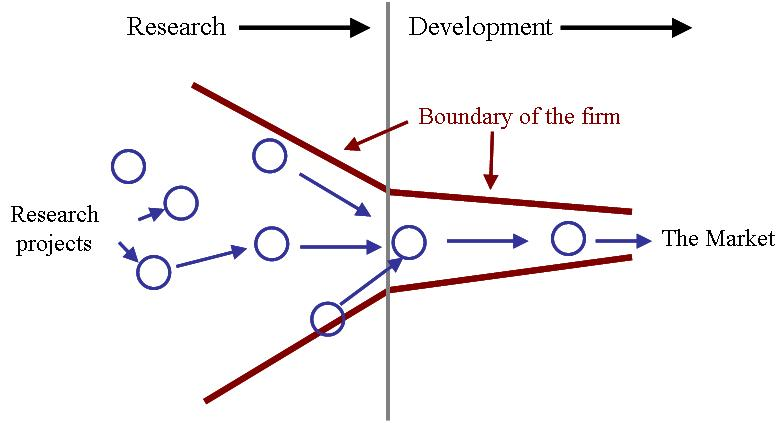
\includegraphics[width=0.8\textwidth]{images/closed_inovations_funnel.jpg}
    \caption{Zatvoreni pristup inoviranju \citep{openinnovation2016}.}\label{fig:closed_inovations_funnel}
\end{figure}

Kao posljedica efekta lijevka mnoge ideje ostanu neiskorištene, ali se dodaju u
bazu znanja tvrtke. Tvrtke koje primjenjuju zatvoreni pristup inoviranju obično
imaju veliku bazu znanja, koja se može koristiti za razvoj novih proizvoda i
usluga \citep{zatvorenaotvorena2020,openinnovation2003}.

Istraživanje i razvoj novih proizvoda i usluga rade dvije skupine ljudi:
\begin{itemize}
    \item istraživači koji razvijaju nove ideje i
    \item inženjeri koji razvijaju nove proizvode i usluge.
\end{itemize}
Istraživači su najčešće jako specijalizirani znanstvenici ili inženjeri,
najčešće s doktoratom. Tvrtke ih vrbuju velikim plaćama i velikom slobodom rada
na projektima. Pošto su istraživači jako specijalizirani teško ih je ponovno
trenirati ako se poslovno stanje promijeni. Inženjeri na drugoj strani su
specijalizirani za rješavanje problema unutar zadanih granica. Uzimaju rezultat
istraživanja i razvijaju proizvod ili uslugu unutar zadanih granica, vrijeme i
budžet \citep{openinnovation2003}.
\chapter{Otvorene inovacije} \label{ch:otvorene_inovacije}

Otvorena inovacija je koncept koji izaziva tradicionalni pristup vertikalnoj
integraciji, gdje interni istraživačko-razvojni (IR\&D) aktivnosti vode internom
razvoju proizvoda koji se potom distribuiraju od strane tvrtke. Umjesto toga,
otvorena inovacija uključuje namjerni unos i izlaz znanja radi ubrzanja interne
inovacije i proširenja tržišta za vanjsko korištenje inovacija, redom
\citep{forbesopeninnovation2011}. Otvorena inovacija je praksa poduzeća i
organizacija da pronalaze ideje iz vanjskih i internih izvora. To znači
dijeljenje znanja i informacija o problemima i traženje rješenja i prijedloga od
ljudi izvan poslovanja \citep{braineetopeninnovation2023}.

\begin{figure}
    \centering
    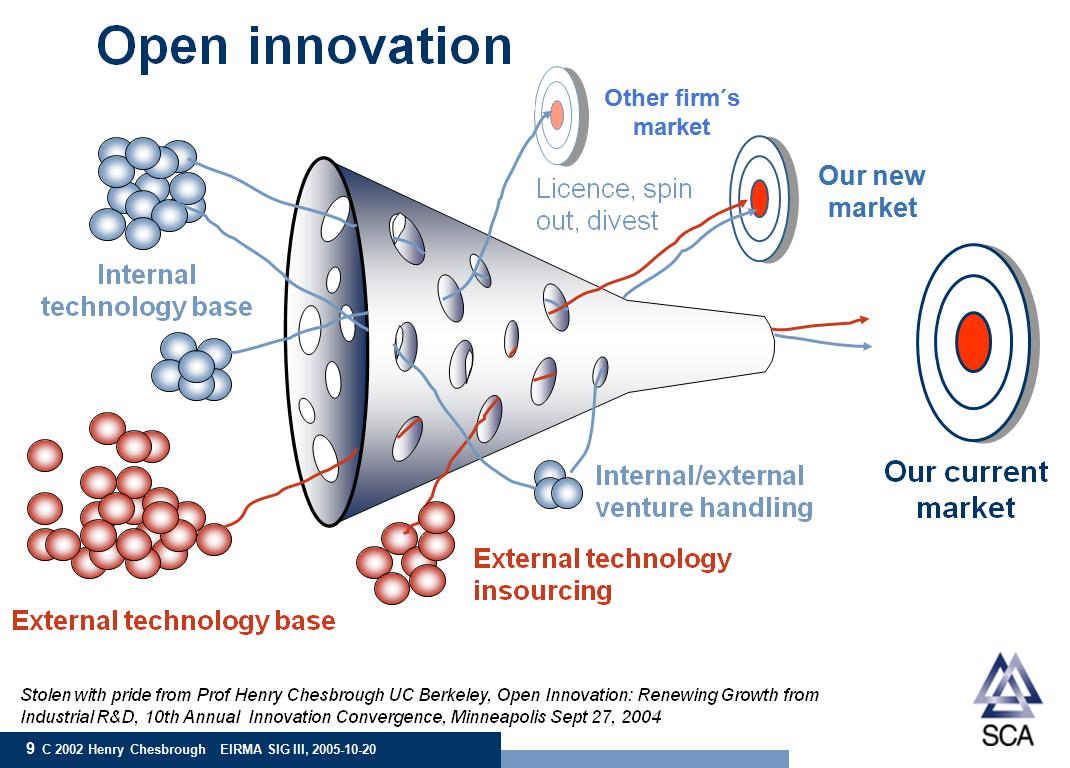
\includegraphics[width=0.8\textwidth]{images/open-innovation11}
    \caption{Prikaz otvorenr inovacije \citep{pakbecopeninnovation2013}.}
    \label{fig:open_innovation}
\end{figure}

Otvorena inovacija se može razumjeti kao antiteza tradicionalnom pristupu
inovaciji. Vanjsko-unutrašnji aspekt se odnosi na unose vanjskih ideja i
tehnologija u vlastiti proces inovacije tvrtke. To je najčešće prepoznata
karakteristika otvorene inovacije. Unutra-vanjski dio je kada neiskorištene ili
nedovoljno iskorištene ideje i tehnologije unutar tvrtke izlaze i inkorporiraju
se u inovacijske procese drugih. Poslovni model je još jedan ključni element
koncepta otvorene inovacije, jer određuje koje ideje i tehnologije treba tražiti
izvana i koje treba pustiti izvan tvrtke \citep{forbesopeninnovation2011}.

Otvorena inovacija nije usmjerena samo na tvrtke; uključuje i kreativne
potrošače i zajednice korisnika-inovatora. Inovacije često dolaze izvana i od
osnivača start-upova, a ne iz postojećih organizacija. Središnja ideja otvorene
inovacije je da u svijetu široko rasprostranjenog znanja tvrtke ne mogu
oslanjati isključivo na vlastita istraživanja, već trebaju kupovati ili
licencirati procese ili izume drugih tvrtki. To se naziva dolaznom otvorenom
inovacijom. Također, interni izumi koji se ne koriste u poslovanju tvrtke
trebaju biti izneseni izvan tvrtke \citep{wikipediaopeninnovation2021}.

Otvorena inovacija nije jednosmjerna ulica. Pozivajući druge da sudjeluju u
generiranju ideja za proizvode i usluge, tvrtke također mogu dijeliti
informacije i stručnost s zajednicama obožavatelja i korisnicima. To stvara
distribuirani, participativniji i decentraliziraniji pristup inovaciji, koji
može otključati mnoge prednosti za poslovanje
\citep{braineetopeninnovation2023}.
\chapter{Usporedba otvorene i zatvorene inovacije} \label{ch:usporedba_otvorene_i_zatvorene_inovacije}

Otvorena inovacija i zatvorena inovacija su dvije različite strategije
upravljanja inovacijama unutar tvrtke. Glavna razlika između ovih pristupa leži
u tome kako se generira inovacija i u kojoj mjeri se uključuje vanjsko znanje u
proces inovacije.

\section{Prednosti i mane otvorenih inovacija} \label{sec:prednosti_i_mane_otvorenih_inovacija}

Otvorena inovacija je suradnički pristup koji omogućuje organizacijama
iskorištavanje vanjskih znanja, vještina i resursa kako bi poboljšale
inovacijske rezultate i otkrile nove ideje (vidi
poglavlje~(\ref{ch:otvorene_inovacije})). Evo nekih prednosti i nedostataka
otvorene inovacije:

\textbf{Prednosti otvorene inovacije}:

\begin{itemize}
\item Proces razvoja inovacija postaje mnogo učinkovitiji i brži \citep{gotechinnovationcompare2021}.
\item Otvorena inovacija može biti ekonomičnija od tradicionalnih metoda \citep{a2dopeninnovation2023}.
\item Otvorena inovacija omogućuje stvarne povratne informacije od raznolikog
skupa ljudi koji nisu ograničeni istim odgovornostima kao zaposlenici unutar
organizacije \citep{a2dopeninnovation2023}.
\item Uključivanje mnoštva omogućava izloženost raznolikom nizu ideja,
prijedloga i perspektiva \citep{a2dopeninnovation2023}.
\item Otvorena inovacija može pomoći organizacijama u identifikaciji novih
talenata \citep{a2dopeninnovation2023}.
\end{itemize}

\textbf{Nedostaci otvorene inovacije:}

\begin{itemize}
\item Otvorenost prema tržištu dovodi do rizika povezanih s procurivanjem
informacija i kibernetičkom sigurnošću \citep{gotechinnovationcompare2021}.
\item Postoje rizici u pogledu donošenja pogrešnog izbora među startupima i
tvrtkama koje nude inovativne proizvode i tehnologije \citep{gotechinnovationcompare2021}.
\item Postoji rizik da talentirani zaposlenici korporativnog tima za inovacije
budu privučeni konkurentskim tvrtkama \citep{gotechinnovationcompare2021}.
\item Pravni aspekti otvorene inovacije često se zanemaruju \citep{timercompare2016}.
\item Otvorena inovacija može se doživljavati kao rizična zbog pitanja
intelektualnog vlasništva \citep{a2dopeninnovation2023}.
\end{itemize}

\section{Prednosti i mane zatvorenih inovacija} \label{sec:prednosti_i_mane_zatvorenih_inovacija}

Zatvorena inovacija, također poznata kao tradicionalna inovacija, odnosi se na
pristup u kojem se nove tehnologije razvijaju s ograničenim korporativnim
resursima i bez vanjske stručnosti (vidi
poglavlje~(\ref{ch:zatvorene_inovacije})). Evo nekih prednosti i nedostataka
zatvorene inovacije:

\textbf{Prednosti zatvorene inovacije:}

\begin{itemize}
\item Korporacija ima potpunu kontrolu nad procesom inovacije i intelektualnim
vlasništvom \citep{asd1}.
\item Korporacija može zadržati povjerljivost poslovnih tajni \citep{asd1}.
\item Korporacija može iskoristiti postojeće resurse i znanje za stvaranje novih
proizvoda \citep{asd2}.
\end{itemize}

\textbf{Nedostaci zatvorene inovacije:}

\begin{itemize}
\item Zatvorena inovacija može rezultirati nedostatkom kreativnosti i inovacije
zbog ograničenog izvora stručnosti i znanja \citep{asd1}.
\item Zatvorena inovacija može biti skupa, jer korporacija mora ulagati u
istraživanje i razvoj te možda ne može iskoristiti vanjske resurse i znanje \citep{asd1}.
\item Korporacija može propustiti vrijedne ideje i povratne informacije iz
vanjskih izvora \citep{asd1}.
\item Zatvorena inovacija može biti spora, jer korporacija se mora osloniti na
vlastite resurse i znanje za razvoj novih proizvoda \citep{asd2}.
\item Korporacija možda neće moći pratiti promjene u trendovima na tržištu \citep{asd2}.
\end{itemize}

\section{Usporedba} \label{sec:usporedba}

Otvorena inovacija i zatvorena inovacija su dvije različite pristupe upravljanju
inovacijama. Zatvorena inovacija se temelji na gledištu da inovacije razvijaju
same tvrtke, pri čemu se inovacijski proces odvija isključivo unutar tvrtke. S
druge strane, otvorena inovacija uključuje vanjska znanja u upravljanje
inovacijama i znači otvaranje inovacijskog procesa izvan granica tvrtke radi
povećanja vlastitog inovacijskog potencijala kroz aktivno strateško korištenje
okruženja \citep{asd3}.

Evo nekih usporedbi između otvorene inovacije i zatvorene inovacije:

\textbf{Proces inovacija:}

U zatvorenoj inovaciji inovacija se razvija u zatvorenom okruženju tvrtke, dok
otvorena inovacija uključuje vanjska znanja u upravljanje inovacijama \citep{asd3}.

\textbf{Kontrola:}

U zatvorenoj inovaciji korporacija ima potpunu kontrolu nad inovacijskim
procesom i intelektualnim vlasništvom, dok u otvorenoj inovaciji korporacija
mora dijeliti kontrolu s vanjskim akterima poput kupaca, dobavljača, sveučilišta
ili drugih tvrtki \citep{asd3}.

\textbf{Kreativnost i inovacija:}

Zatvorena inovacija može rezultirati nedostatkom kreativnosti i inovacije zbog
ograničenog izvora stručnosti i znanja, dok otvorena inovacija omogućuje stvarne
povratne informacije od raznolikog skupa ljudi koji nisu ograničeni istim
odgovornostima kao zaposlenici unutar organizacije \citep{asd3}.

\textbf{Trošak:}

Otvorena inovacija može biti ekonomičnija od zatvorene inovacije jer omogućuje
organizacijama da iskoriste vanjska znanja, vještine i resurse kako bi
poboljšale inovacijske rezultate i otkrile nove ideje \citep{asd3}.

\textbf{Intelektualno vlasništvo:}

Zatvorena inovacija može zadržati povjerljivost poslovnih tajni i zaštititi
intelektualno vlasništvo, dok otvorena inovacija uključuje dijeljenje znanja i
može uključivati visoke troškove za korištenje licenci i drugih oblika
intelektualnog vlasništva \citep{asd3}.

\textbf{Konkurencija:}

Zatvorena inovacija možda neće moći pratiti promjene u trendovima na tržištu i
konkurenciju, dok otvorena inovacija organizacijama omogućuje pristup raznolikim
znanjima i vještinama za razvoj inovativnih proizvoda ili usluga koji im mogu
pomoći ostati konkurentni \citep{asd4}.

Zaključno, otvorena inovacija i zatvorena inovacija su dva različita pristupa
upravljanju inovacijama, s različitim prednostima i nedostacima. Zatvorena
inovacija pruža kontrolu nad inovacijskim procesom i intelektualnim vlasništvom,
ali može rezultirati nedostatkom kreativnosti i inovacije zbog ograničenih
resursa i znanja. Otvorena inovacija organizacijama omogućuje pristup raznolikom
znanju i vještinama, ubrzava vrijeme dolaska na tržište i smanjuje troškove, ali
također nosi rizike poput procurivanja informacija i mogućnosti donošenja
pogrešnih odluka među startupima i tvrtkama koje nude inovativne proizvode i
tehnologije. Važno je procijeniti potrebe i resurse organizacije prije donošenja
odluke o odabiru zatvorene ili otvorene inovacijske strategije \citep{asd3}.
\chapter{Plasiranje inovacije} \label{plasiranje_inovacije}



\chapter{Zaključak}
Zaključak.

\bibliography{literatura}
\bibliographystyle{ieeetr}

\end{document}
